%\documentclass[handout]{beamer}
\documentclass[t,french]{beamer}
\usepackage{babel}
\usepackage[latin1]{inputenc}
\usepackage{graphicx} %for jpg files
\usepackage{beamerthemesplit} % new 
\usetheme[compress]{Berlin}
\usecolortheme{beaver}
\usepackage{tikz}%tikz figures
\usetikzlibrary{shapes}
\usepackage{pgffor}% http://ctan.org/pkg/pgffor
\usepackage{multirow}
\usepackage{ifthen}
\usepackage{subfigure} %spacing for table of contents
\usepackage{boolexpr}
\usepackage{movie15}
\usepackage{amsmath}
\usepackage{amsfonts}
\usepackage{amssymb}
\usepackage{hyperref}
\usepackage{listings}
%\usepackage{enumitem}
%\setitemize{itemsep=1.5em,%
%  label=\usebeamerfont*{itemize item}%
%        \usebeamercolor[fg]{itemize item}%
%        \usebeamertemplate{itemize item}%
%}
%
%
%\usepackage{bbold}
%\usepackage{multimedia} %videos inside frame
%
%
\graphicspath{{images/}}

\def\R{ \ensuremath{\mathcal{R}} }
\def\C{ \ensuremath{\mathcal{C}} }
\def\SV{ \ensuremath{\mathcal{SV}} }

\setbeamercolor{alerted text}{fg=orange}
\setbeamercolor{background canvas}{bg=white}
\setbeamercolor{block body alerted}{bg=normal text.bg!90!black}
\setbeamercolor{block body}{bg=normal text.bg!90!black}
\setbeamercolor{block body example}{bg=normal text.bg!90!black}
\setbeamercolor{block title}{bg=blue}
\setbeamercolor{fine separation line}{}
\setbeamercolor{frametitle}{fg=black,bg=gray!30}
\setbeamercolor{item projected}{fg=black}
\setbeamercolor{normal text}{bg=black,fg=black}
\setbeamercolor{palette sidebar primary}{use=normal text,fg=normal text.fg}
\setbeamercolor{palette sidebar quaternary}{use=structure,fg=structure.fg}
\setbeamercolor{palette sidebar secondary}{use=structure,fg=structure.fg}
\setbeamercolor{palette sidebar tertiary}{use=normal text,fg=normal text.fg}
\setbeamercolor{section in sidebar}{fg=black}
\setbeamercolor{section in sidebar shaded}{fg= grey}
\setbeamercolor{separation line}{}
\setbeamercolor{sidebar}{bg=red}
\setbeamercolor{sidebar}{parent=palette primary}
\setbeamercolor{structure}{bg=black, fg=red}
\setbeamercolor{subsection in sidebar}{fg=black}
\setbeamercolor{subsection in sidebar shaded}{fg=grey}
\setbeamercolor{title}{fg=black!100,bg=gray!30}
\setbeamercolor{titlelike}{fg=brown}

%several template parameters
\setbeamertemplate{frametitle}[default][center]
\setbeamertemplate{blocks}[rounded][shadow=true]
%\beamertemplateshadingbackground{white!20}{black!20}
\setbeamertemplate{background canvas}[vertical shading][bottom=white,top=white!25]
\setbeamertemplate{sidebar canvas left}[horizontal shading][left=white!40!black,right=black]
\setbeamercolor{footline in sidebar}{fg=black}%[page number]
%\setbeamertemplate{footline}[frame number]
%suppress navigational bar
\beamertemplatenavigationsymbolsempty
%experimental stuff
\setbeamertemplate{title page}[default][rounded=true,shadow=true]


% Images
\pgfdeclareimage[width=10cm]{ROSEquation}{./images/ros_equation_2}
\pgfdeclareimage[width=10cm]{gazebo}{./images/gazebo_horz_cmyk_pos.jpg}
\pgfdeclareimage[width=10cm]{opencv}{./images/opencv_logo.png}
\pgfdeclareimage[width=10cm]{pcl}{./images/pointcloudlibrary_horz_large_pos.jpg}
\pgfdeclareimage[width=10cm]{moveit}{./images/moveit-logo.png}

% Tikz libraries
\usetikzlibrary{shadows}
\usetikzlibrary{automata}
\usetikzlibrary{arrows}

% For arrows
\definecolor{darkblue}{rgb}{0.2,0.2,0.6}
\definecolor{darkred}{rgb}{0.6,0.1,0.1}
\definecolor{darkgreen}{rgb}{0.2,0.6,0.2}

\def\arrowt{
  (0.1,0.5) -- (0.0,1) -- (6.0,1.0) [rounded corners=0.5] --
  (6.0,1.5) [rounded corners=1] -- (7.0,0.5) [rounded corners=0.5] --
  (6.0,-0.5) [sharp corners] -- (6.0,0.0) -- (0.0,0.0)
  [rounded corners=1] -- (0.1,0.5) -- cycle
}

\def\arrowd{
  (10.75:1.1) -- (6.5:1) arc (6.25:120:1) [rounded corners=0.5] --
  (120:0.9) [rounded corners=1] -- (130:1.1) [rounded corners=0.5] --
  (120:1.3) [sharp corners] -- (120:1.2) arc (120:5.25:1.2)
  [rounded corners=1] -- (10.75:1.1) -- (6.5:1) -- cycle
}

\def\arrow{
  (10.75:1.1) -- (6.5:1) arc (6.25:90:1) [rounded corners=0.5] --
  (90:0.9) [rounded corners=1] -- (100:1.1) [rounded corners=0.5] --
  (90:1.3) [sharp corners] -- (90:1.2) arc (90:5.25:1.2)
  [rounded corners=1] -- (10.75:1.1) -- (6.5:1) -- cycle
}

\def\arrowtd{
  (-10.75:1.1) -- (-6.5:1) arc (-6.25:-170:1) [rounded corners=0.5] --
  (-170:0.9) [rounded corners=1] -- (-180:1.1) [rounded corners=0.5] --
  (-170:1.3) [sharp corners] -- (-170:1.2) arc (-170:-5.25:1.2)
  [rounded corners=1] -- (-10.75:1.1) -- (-6.5:1) -- cycle
}

\tikzset{
  ashadow/.style={opacity=.25, shadow xshift=0.07, shadow yshift=-0.07},
}


\def\arrows[#1]{         
  \begin{scope}[scale=#1]
    \draw[color=darkred, %
    drop shadow={ashadow, color=red!60!black}] \arrow;

    %\draw[color=darkgreen, bottom color=green!90!black, top color=green!60, %
    %drop shadow={ashadow, color=green!60!black}] [rotate=120] \arrow;

    %\draw[color=darkblue, right color=blue, left color=blue!60, %
    %drop shadow={ashadow, color=blue!60!black}] [rotate=240] \arrow;

    % to hide the green shadow

  \end{scope}
}

\include{commands}

\setlength{\unitlength}{\textwidth}  % measure in textwidths
\begin{document}

\title{Introduction ROS}

\author{Olivier Stasse \\ LAAS-CNRS, Toulouse, France}
%-- \insertframenumber/\inserttotalframenumber}

\date{20-21/05/2014} 

\AtBeginSection[]
{
  \begin{frame}
    \frametitle{Table des mati�res}
    \tableofcontents[currentsection,
      hideothersubsections]
  \end{frame}
}
%%%%%%%%%%%%%%%%%%%%%%%%%%%%%%%%%%%%%%%%%%%%%%%%%%%%%%%%%%%%%%%%%%%%%%%%%%%%%%%
{
  \usebackgroundtemplate{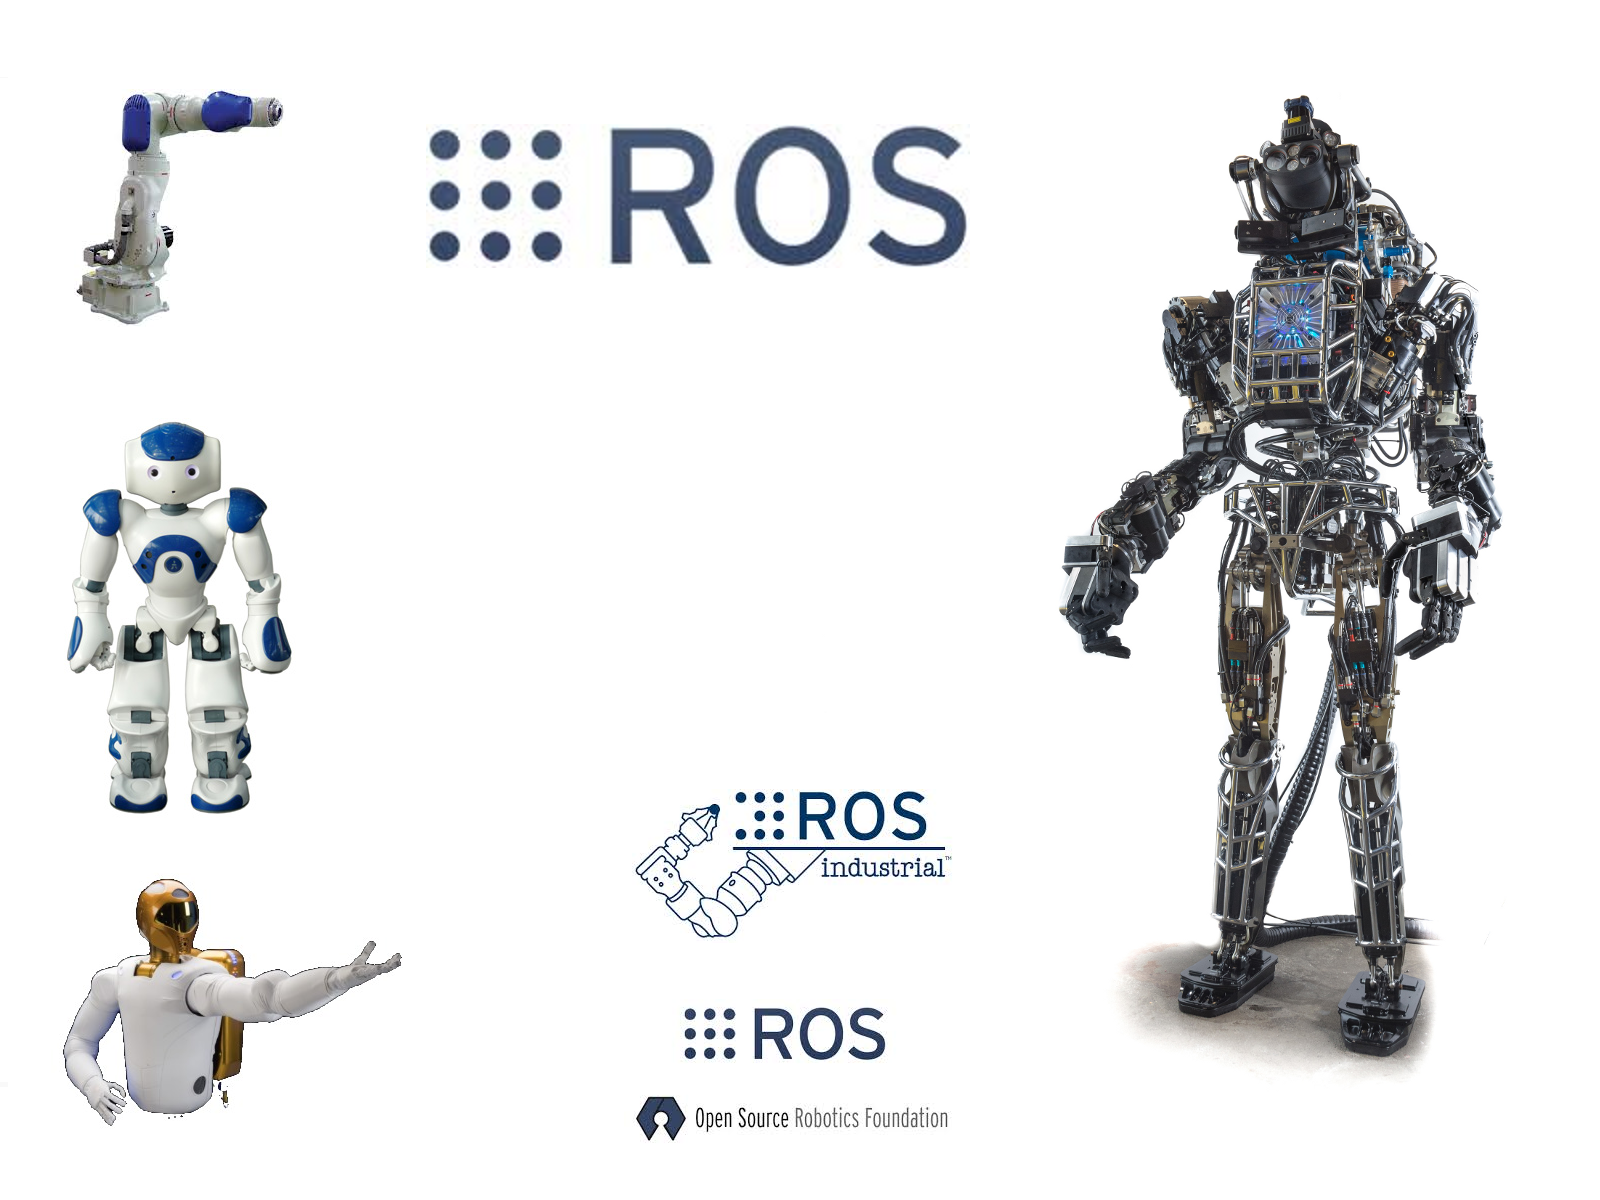
\includegraphics[width=1.0\paperwidth]{images/background-title-3.png}}
  \begin{frame}[plain]
    %\tikzstyle{stringbox}=[rectangle,color=black,fill=blue!10,text=black,draw,text opacity=0.4,align=flush center]
    \begin{tikzpicture}[remember picture, overlay]
       \node [yshift=1.8cm, xshift=-1cm, text width=4cm] (title) at (current page.center) 
             { Etude de cas \\
              sur HRP-2};
       \node [xshift=-3.1cm,yshift=0.5cm,
              fill=white!10,fill opacity=0.7,right,text width=3cm]
            (author) at (current page.center) [scale=0.7]
            {  Olivier STASSE, \\
              CR-1, CNRS, \\
              Gepetto, \\
              LAAS CNRS }; 
       \node [xshift=-3.1cm,yshift=-0.8cm,
              fill=white!10,fill opacity=0.7,
              right,text width=3cm]
        (author) 
        at (current page.center)
            {
              AIP, Toulouse\\
              $20-21$ Mai
              2014
            }; 
    \end{tikzpicture}
  \end{frame}
}
\begin{frame}
  \frametitle{Table des mati�res}
  \tableofcontents
\end{frame}
%%%%%%%%%%%%%%%%%%%%%%%%%%%%%%%%%%%%%%%%%%%%%%%%%%%%%%%%%%%%%%%%%%%%%%%%%%%%%%%
\section{Motivations}
\begin{frame}{HRP-2 et ROS}
  \begin{block}{Contraintes}
    \begin{itemize}
      \item HRP-2 utilise un autre middleware Corba - OpenRTM
      \item La structure de contr�le bas-niveau du robot est binairement li� � ce middleware.
      \item Le simulateur utilis� est partiellement Open-Source mais
        particuli�rement adapt�.
      \item L'OS temps r�el du robot est tout � fait satisfaisant.
    \end{itemize}
  \end{block}
  \begin{alertblock}{Probl�me}
    Interfacer ROS (non temps r�el) avec l'architecture de contr�le.
  \end{alertblock}
\end{frame}
%%%%%%%%%%%%%%%%%%%%%%%%%%%%%%%%%%%%%%%%%%%%%%%%%%%%%%%%%%%%%%%%%%%%%%%%%%%%%%%
\begin{frame}{HRP-2 - la structure sp�cifique du robot}
  \begin{figure}
    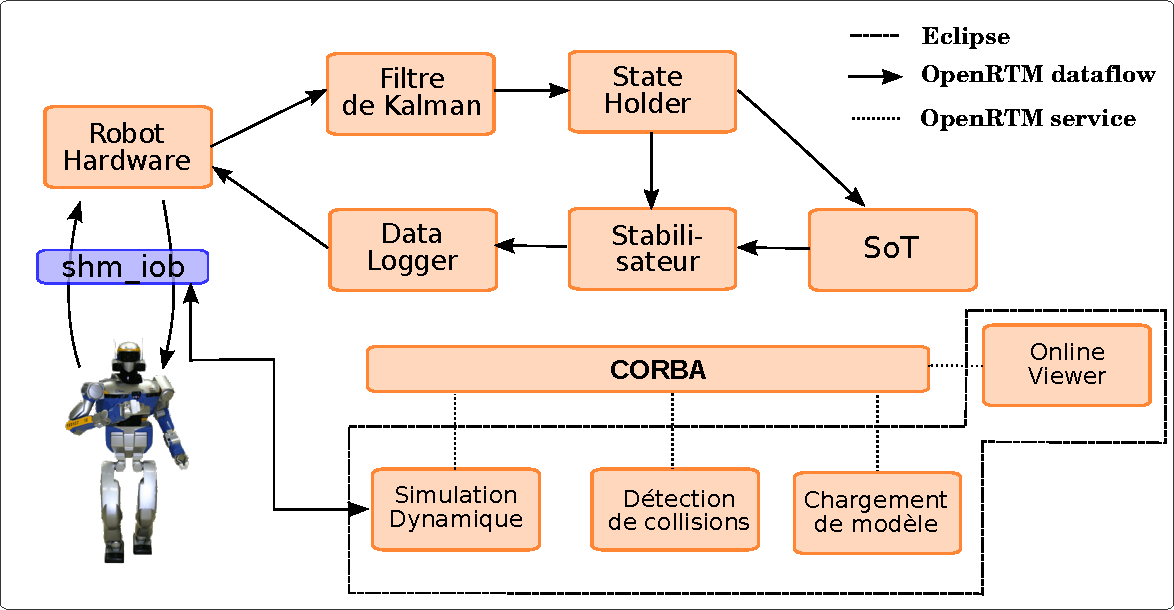
\includegraphics[width=0.9\linewidth]{./images/Concept-Software-HRP-2}
  \end{figure}
\end{frame}
%%%%%%%%%%%%%%%%%%%%%%%%%%%%%%%%%%%%%%%%%%%%%%%%%%%%%%%%%%%%%%%%%%%%%%%%%%%%%%%
\begin{frame}{HRP-2 - Adaptation � ROS}
  \begin{figure}
    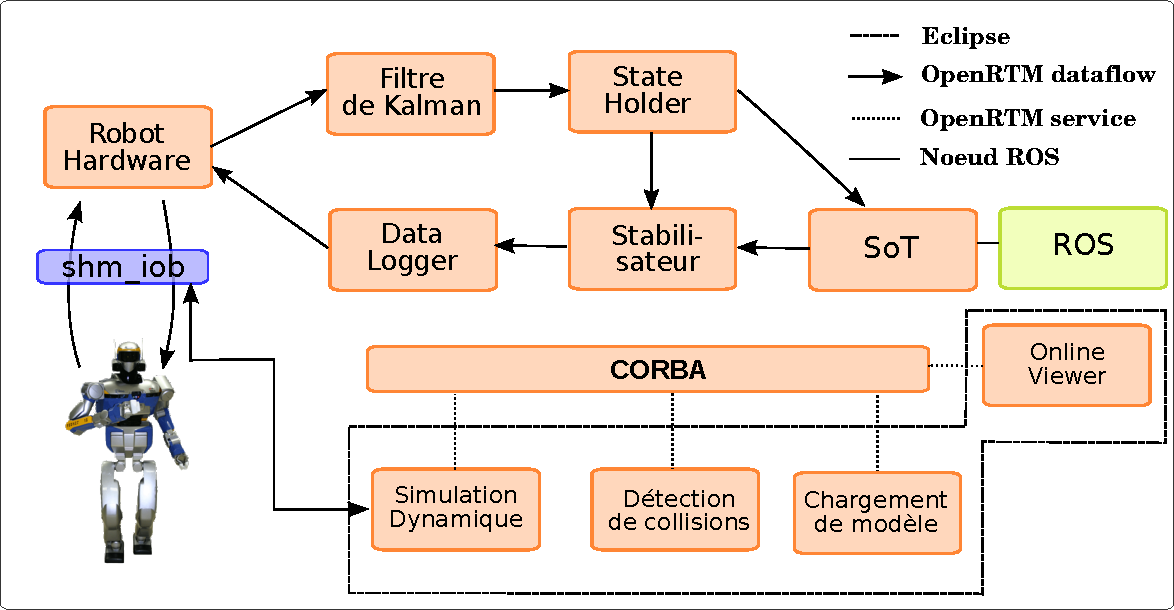
\includegraphics[width=0.9\linewidth]{./images/Concept-Software-HRP-2-ROS}
  \end{figure}
\end{frame}
%%%%%%%%%%%%%%%%%%%%%%%%%%%%%%%%%%%%%%%%%%%%%%%%%%%%%%%%%%%%%%%%%%%%%%%%%%%%%%%
%%%%%%%%%%%%%%%%%%%%%%%%%%%%%%%%%%%%%%%%%%%%%%%%%%%%%%%%%%%%%%%%%%%%%%%%%%%%%%%
%%%%%%%%%%%%%%%%%%%%%%%%%%%%%%%%%%%%%%%%%%%%%%%%%%%%%%%%%%%%%%%%%%%%%%%%%%%%%%%

\section{Structure du logiciel de contr�le}
%
\begin{frame}{Structure logicielle du contr�le - Sch�ma conceptuel}
  \begin{figure}
    \includegraphics[width=\linewidth]{./images/Concept-Fig}
  \end{figure}
\end{frame}
%%%%%%%%%%%%%%%%%%%%%%%%%%%%%%%%%%%%%%%%%%%%%%%%%%%%%%%%%%%%%%%%%%%%%%%%%%%%%%%
\begin{frame}{Structure logicielle du contr�le - Sch�ma conceptuel}
  \begin{figure}
    \includegraphics[width=\linewidth]{./images/Concept-Theory-Fig-Finalv2M5}
  \end{figure}
\end{frame}
%%%%%%%%%%%%%%%%%%%%%%%%%%%%%%%%%%%%%%%%%%%%%%%%%%%%%%%%%%%%%%%%%%%%%%%%%%%%%%%
\begin{frame}{Structure logicielle du contr�le - Sch�ma conceptuel}
  \begin{figure}
    \includegraphics[width=\linewidth]{./images/Concept-Theory-Fig-Finalv2M4}
  \end{figure}
\end{frame}
%%%%%%%%%%%%%%%%%%%%%%%%%%%%%%%%%%%%%%%%%%%%%%%%%%%%%%%%%%%%%%%%%%%%%%%%%%%%%%%
\begin{frame}{Structure logicielle du contr�le - Sch�ma conceptuel}
  \begin{figure}
    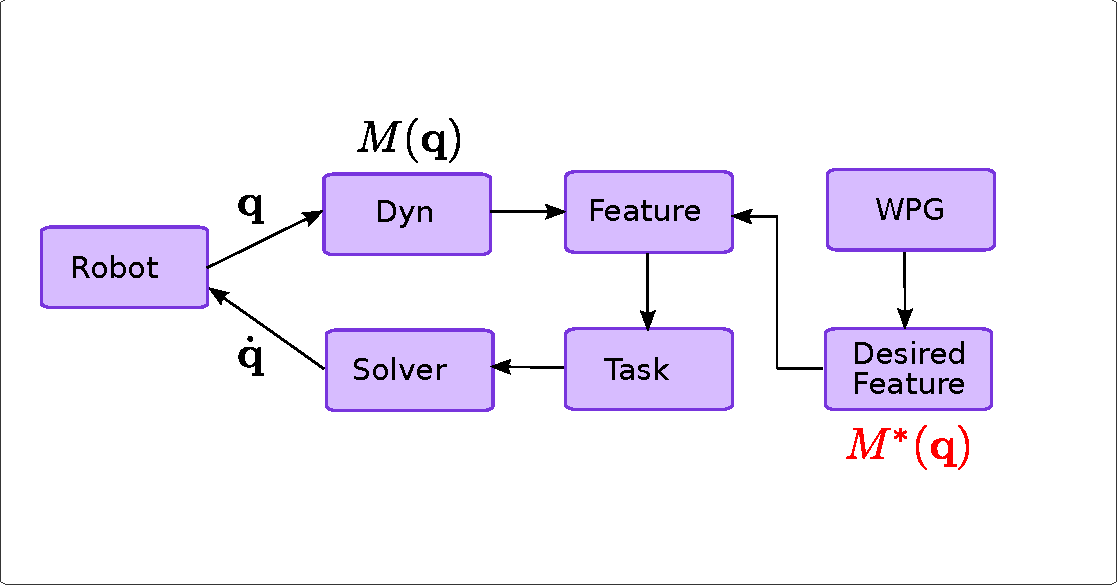
\includegraphics[width=\linewidth]{./images/Concept-Theory-Fig-Finalv2M3}
  \end{figure}
\end{frame}
%%%%%%%%%%%%%%%%%%%%%%%%%%%%%%%%%%%%%%%%%%%%%%%%%%%%%%%%%%%%%%%%%%%%%%%%%%%%%%%
\begin{frame}{Structure logicielle du contr�le - Sch�ma conceptuel}
  \begin{figure}
    \includegraphics[width=\linewidth]{./images/Concept-Theory-Fig-Finalv2M2}
  \end{figure}
\end{frame}
%%%%%%%%%%%%%%%%%%%%%%%%%%%%%%%%%%%%%%%%%%%%%%%%%%%%%%%%%%%%%%%%%%%%%%%%%%%%%%%
\begin{frame}{Structure logicielle du contr�le - Sch�ma conceptuel}
  \begin{figure}
    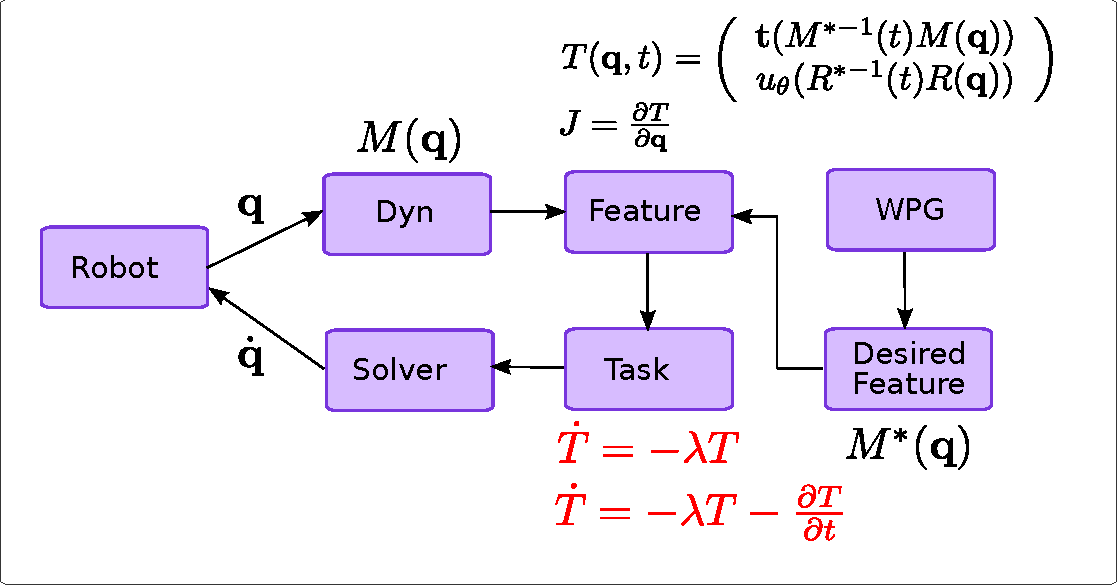
\includegraphics[width=\linewidth]{./images/Concept-Theory-Fig-Finalv2M1}
  \end{figure}
\end{frame}
%%%%%%%%%%%%%%%%%%%%%%%%%%%%%%%%%%%%%%%%%%%%%%%%%%%%%%%%%%%%%%%%%%%%%%%%%%%%%%%
\begin{frame}{Structure logicielle du contr�le - Sch�ma conceptuel}
  \begin{figure}
    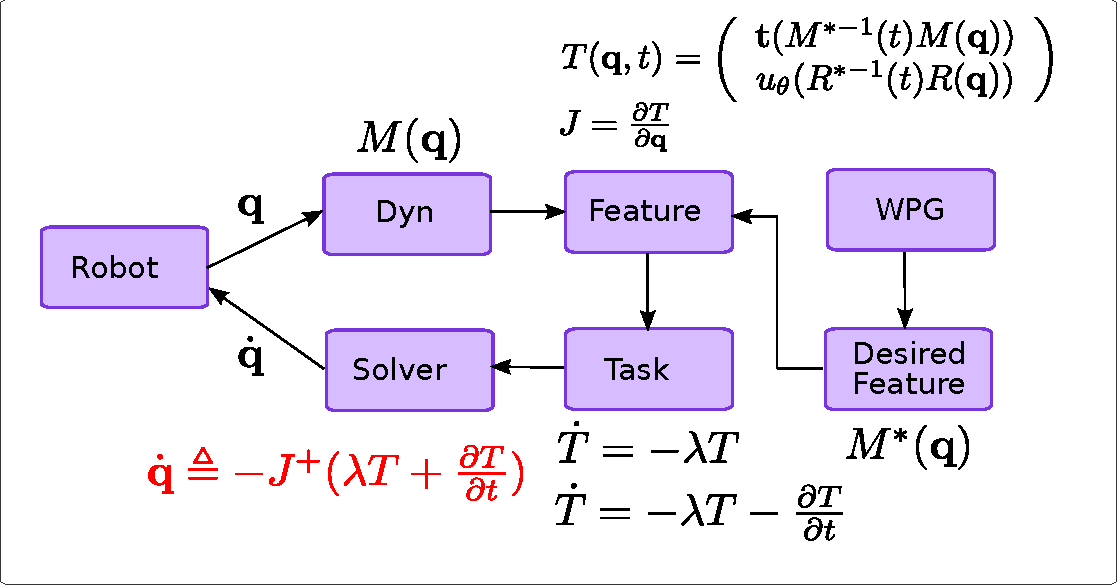
\includegraphics[width=\linewidth]{./images/Concept-Theory-Fig-Finalv2}
  \end{figure}
\end{frame}
%%%%%%%%%%%%%%%%%%%%%%%%%%%%%%%%%%%%%%%%%%%%%%%%%%%%%%%%%%%%%%%%%%%%%%%%%%%%%%%
%\begin{frame}{Software structure - Repositories}
%  \begin{figure}
%    \includegraphics[width=\linewidth]{./images/Concept-Software-Fig}
%  \end{figure}
%\end{frame}
\section{Application}
\begin{frame}{Preuve de Concept - Airbus - HRP-2 dans l'usine du futur}
  \begin{center}
  \href{run:/home/ostasse/Videos/Airbus/PocAirbus2013_12_Short.mp4}
       {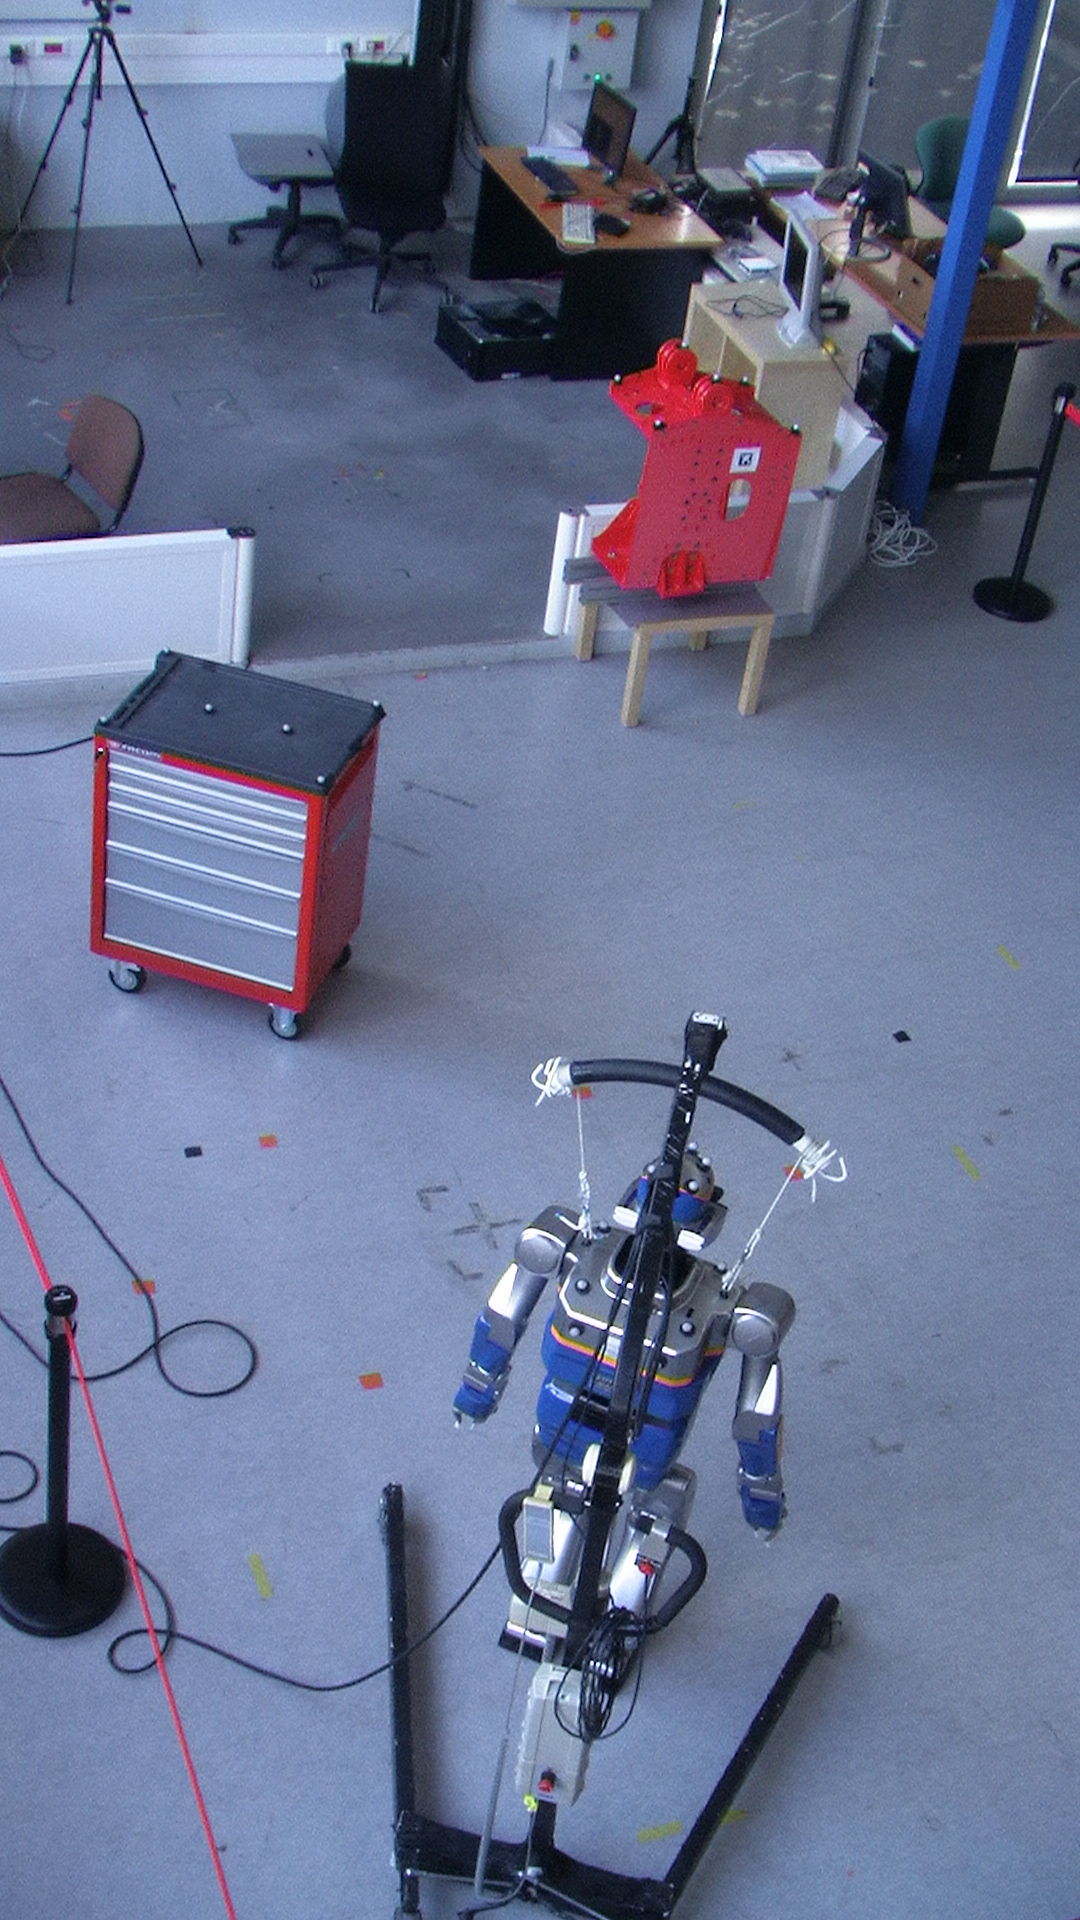
\includegraphics[width=0.4\linewidth]{./images/SituationFastPlanning_2.JPG}}
  \end{center}
\end{frame}
%%%%%%%%%%%%%%%%%%%%%%%%%%%%%%%%%%%%%%%%%%%%%%%%%%%%%%%%%%%%%%%%%%%%%%%%%%%%%%%
\begin{frame}{Structure de l'application - Fast Planning}
  \begin{figure}
    \includegraphics[width=\linewidth]{./images/Concept-Software-HRP-2-ROS-ONLY}
  \end{figure}
\end{frame}
%%%%%%%%%%%%%%%%%%%%%%%%%%%%%%%%%%%%%%%%%%%%%%%%%%%%%%%%%%%%%%%%%%%%%%%%%%%%%%%
\begin{frame}{Structure de l'application - VISP - Screwing}
  \begin{figure}
    \includegraphics[width=\linewidth]{./images/Concept-Software-HRP-2-ROS-VISP}
  \end{figure}
\end{frame}
%%%%%%%%%%%%%%%%%%%%%%%%%%%%%%%%%%%%%%%%%%%%%%%%%%%%%%%%%%%%%%%%%%%%%%%%%%%%%%%
\begin{frame}{Structure des roslaunch}
  \begin{itemize}
    \item Utilisation des inclusions successives des roslaunch:
      \begin{itemize}
        \item \textbf{hrp2\_bringup/openhrp\_bridge.launch}\\
          
          \begin{itemize}
            \item \textbf{hrp2\_bringup/common.launch}
          \end{itemize}
          Lance les noeuds suivants:
          \begin{itemize}       
            \item \textbf{robot\_pose\_ekf/robot\_pose\_ekf}
            \item \textbf{tf2\_ros/buffer\_server}
            \item \textbf{openhrp\_bridge/openhrp\_manager}
          \end{itemize}
        \item \textbf{feasibility/launch/feasibility.launch}\\
          Lance le noeud suivant: \textbf{feasibility/FastReplanner}
      \end{itemize}
    \item Lancement de multiples noeuds:
      \begin{itemize}
        \item \textbf{evart\_bridge/evart}
        \item \textbf{airbus\_demonstrator/launcher}
      \end{itemize}
  \end{itemize}
\end{frame}

%%%%%%%%%%%%%%%%%%%%%%%%%%%%%%%%%%%%%%%%%%%%%%%%%%%%%%%%%%%%%%%%%%%%%%%%%%%%%%%
%%%%%%%%%%%%%%%%%%%%%%%%%%%%%%%%%%%%%%%%%%%%%%%%%%%%%%%%%%%%%%%%%%%%%%%%%%%%%%%
%%%%%%%%%%%%%%%%%%%%%%%%%%%%%%%%%%%%%%%%%%%%%%%%%%%%%%%%%%%%%%%%%%%%%%%%%%%%%%%
\end{document}


